
% Start and ice-breaker:

% Introducing myself





\begin{frame}{Introducing Myself}
   \begin{block}{Education}
    \begin{itemize}
     \item Master's Degrees in Microelectronics and Mathematics
     \item Doctoral Degree in Microelectronics
     \item Home University: TU Wien
    \end{itemize}

   \vspace*{-2cm}
   \begin{flushright}
     
\includegraphics[width=0.15\textwidth]{figures/TU-Signet}
   \end{flushright}

   \end{block}



   \begin{block}{Interests}
    \begin{itemize}
     \item Efficient Numerics on Modern Hardware
     \item High-level APIs
     \item Semiconductor Device Simulation
    \end{itemize}

   \end{block}

   \begin{block}{Contact}
    \begin{itemize}
     \item Email: rupp@mcs.anl.gov
     \item Web: http://www.karlrupp.net/
     \item Find me at: Google+, Twitter, LinkedIn
    \end{itemize}
   \end{block}

\end{frame}






\begin{frame}{Before we start...}

   \begin{block}{Goal of this Workshop}
    \begin{itemize}
     \item {\Huge \textbf{\color{red} You}} should learn new things about HPC
    \end{itemize}
   \end{block}

   \vspace*{1cm}
   \begin{block}{Ask Questions}
    \begin{itemize}
     \item Tell me if you do not understand
     \item Ask for further details
     \item Don't be shy
    \end{itemize}
   \end{block}

\end{frame}



%%%%%% General PETSc information %%%%%%%%%%

%%% What is PETSc

%
% Stats, Who, Philosophy
%




\section{PETSc Overview}
\begin{frame}{PETSc}
   \begin{center} \Large \textbf{About PETSc} \end{center}
\end{frame}

\begin{frame}[fragile]
\frametitle{PETSc Origins}
 
 \begin{center} \LARGE
  \definecolor{ddviolet}{rgb}{0.561, 0.067, 0.455}  % RGB 143-17-116
  PETSc was developed as a Platform for \\[0.2em] \textbf{\color{ddviolet} Experimentation}
 \end{center}

 \vspace{1cm}
 \begin{block}{We want to experiment with different}
 \begin{itemize}
  \item Models
  \item Discretizations
  \item Solvers
  \item Algorithms
 \end{itemize}
 \end{block}

 \begin{block}{These boundaries are often blurred...}
 \end{block}

 \begin{flushright}
  \vspace*{-5cm}
  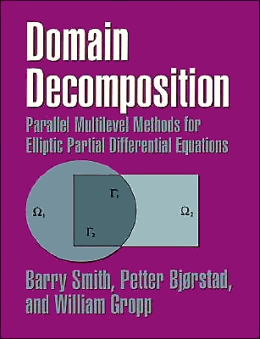
\includegraphics[width=0.4\textwidth]{dd-book-smith.png}
 \end{flushright}

\end{frame}




\newcommand\ganttline[4]{% line, tag, start end
   \node at (0,#1/2+.1) [anchor=base east] {#2};
   \fill[blue] (#3/\xtick-1991/\xtick,#1/2-.1) rectangle (#4/\xtick-1991/\xtick,#1/2+.1);}
\newcommand\ganttlabel[6]{% year, label, color, yloc, anchor
  \node[#3] at (#1/\xtick+#6/\xtick-1991/\xtick,#4) [anchor=#5] {#2};
  \fill[#3] (#1/\xtick-1991/\xtick,1/2-.1) rectangle (#1/\xtick-1991/\xtick+0.04,15/2+.1);}

\begin{frame}{Timeline}
%\frame{
\begin{figure}[htbp]
\vspace*{-0.4cm}
\hspace*{-0.8cm}
\def\present{2016.2}
\def\xtick{2.8}
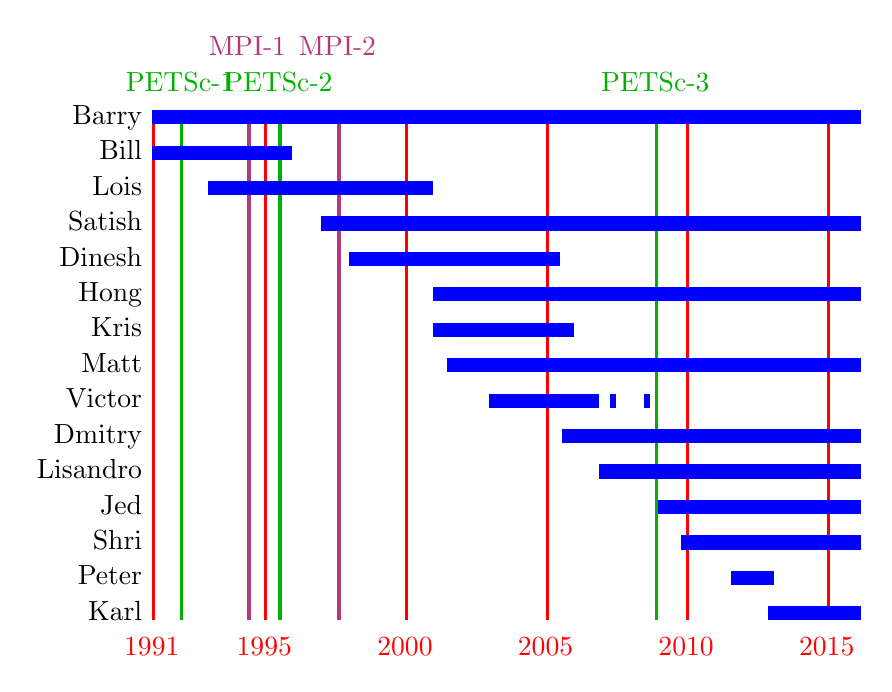
\begin{tikzpicture}[y=-0.9cm]
   %\draw[help lines] (0.5,5) grid (8,0.5);
   \ganttlabel{1991}{1991}{red}{7.7}{north}{0}
   \ganttlabel{1995}{1995}{red}{7.7}{north}{0}
   \ganttlabel{2000}{2000}{red}{7.7}{north}{0}
   \ganttlabel{2005}{2005}{red}{7.7}{north}{0}
   \ganttlabel{2010}{2010}{red}{7.7}{north}{0}
   \ganttlabel{2015}{2015}{red}{7.7}{north}{0}
   \ganttlabel{1992}{PETSc-1}{green!70!black}{0}{center}{0}
   \ganttlabel{1994.4}{MPI-1}{magenta!70!black}{-.5}{center}{0}
   \ganttlabel{1997.6}{MPI-2}{magenta!70!black}{-.5}{center}{0}
   \ganttlabel{1995.5}{PETSc-2}{green!70!black}{0}{center}{0}
   \ganttlabel{2008.9}{PETSc-3}{green!70!black}{0}{center}{0}
   \ganttline{1}{Barry}{1991}{\present}
   \ganttline{2}{Bill}{1991}{1996}
   \ganttline{3}{Lois}{1993}{2001}
   \ganttline{4}{Satish}{1997}{\present}
   \ganttline{5}{Dinesh}{1998}{2005.5}
   \ganttline{6}{Hong}{2001}{\present}
   \ganttline{7}{Kris}{2001}{2006}
   \ganttline{8}{Matt}{2001.5}{\present}
   \ganttline{9}{Victor}{2003}{2006.9}
   \ganttline{9}{}{2007.3}{2007.5}
   \ganttline{9}{}{2008.5}{2008.7}
   \ganttline{10}{Dmitry}{2005.6}{\present}
   \ganttline{11}{Lisandro}{2006.9}{\present}
   \ganttline{12}{Jed}{2009}{\present}
   \ganttline{13}{Shri}{2009.8}{\present}
   \ganttline{14}{Peter}{2011.6}{2013.12}
   \ganttline{15}{Karl}{2012.9}{\present}
\end{tikzpicture}
\end{figure}
%}
\end{frame}

\begin{frame}{PETSc}
\vspace*{-0.2cm}
\begin{center} {\bf Portable} Extensible Toolkit for Scientific Computing \end{center}
\vspace*{-0.2cm}
\begin{block}{Architecture}
    \begin{itemize}  \vspace*{-0.2cm}
    \item tightly coupled (e.g. XT5, BG/P, Earth Simulator)
    \item loosely coupled such as network of workstations
    \item GPU clusters (many vector and sparse matrix kernels)
    \end{itemize}
\end{block} \vspace*{-0.2cm}

\begin{block}{Software Environment}
  \begin{itemize}\vspace*{-0.2cm}
   \item Operating systems (Linux, Mac, Windows, BSD, proprietary Unix)
   \item Any compiler
   \item Usable from C, C++, Fortran 77/90, Python, and MATLAB
   \item Real/complex, single/double/quad precision, 32/64-bit int
  \end{itemize}
\end{block}\vspace*{-0.2cm}

\begin{block}{System Size}
  \begin{itemize}\vspace*{-0.2cm}
   \item 500B unknowns, 75\% weak scalability on Jaguar (225k cores) \\
    and Jugene (295k cores)
   \item Same code runs performantly on a laptop
  \end{itemize}
\end{block}\vspace*{-0.2cm}


\begin{block}{Free to everyone (BSD-style license), open development}\end{block} \vspace*{-0.4cm}

\end{frame}


\begin{frame}{PETSc}

\begin{center}Portable {\bf Extensible} Toolkit for Scientific Computing \end{center}

\begin{block}{Philosophy: Everything has a plugin architecture}
\begin{itemize}
  \item Vectors, Matrices, Coloring/ordering/partitioning algorithms
  \item Preconditioners, Krylov accelerators
  \item Nonlinear solvers, Time integrators
  \item Spatial discretizations/topology$^*$
\end{itemize}

\end{block}

\begin{block}{Example}
  \begin{itemize}
   \item Vendor supplies matrix format and associated preconditioner, distributes
	compiled shared library.  
   \item Application user loads plugin at runtime, no source
	code in sight.
  \end{itemize}
\end{block}

 \vspace{2cm}
\end{frame}


\begin{frame}{PETSc}

\begin{center} Portable Extensible {\bf Toolkit} for Scientific Computing \end{center}

\begin{block}{Toolset}
  \begin{itemize}
   \item algorithms
   \item (parallel) debugging aids
   \item low-overhead profiling
  \end{itemize}
\end{block}

\begin{block}{Composability}
 \begin{itemize}
  \item try new algorithms by choosing from product space
  \item composing existing algorithms (multilevel, domain decomposition, splitting)
 \end{itemize}
\end{block}

\begin{block}{Experimentation}
\begin{itemize}
  \item Impossible to pick the solver \emph{a priori}
  \item PETSc's response: expose an algebra of composition
  \item keep solvers decoupled from physics and discretization
\end{itemize}
\end{block}
\end{frame}

\begin{frame}{PETSc}
\vspace*{-0.2cm}
\begin{center}
 Portable Extensible Toolkit for {\bf Scientific Computing}
\end{center}
\vspace*{-0.2cm}

  \begin{block}{Computational Scientists}
    \begin{itemize}\vspace*{-0.2cm}
    \item PyLith (CIG), Underworld (Monash), Magma Dynamics (LDEO, Columbia), PFLOTRAN (DOE), SHARP/UNIC (DOE)
    \end{itemize}
  \end{block}\vspace*{-0.2cm}
  
  \begin{block}{ Algorithm Developers (iterative methods and preconditioning)} \end{block}\vspace*{-0.4cm}
  
  \begin{block}{ Package Developers}
    \begin{itemize} \vspace*{-0.2cm}
    \item SLEPc, TAO, Deal.II, Libmesh, FEniCS, PETSc-FEM, MagPar, OOFEM, FreeCFD, OpenFVM
    \end{itemize}
  \end{block}\vspace*{-0.2cm}
  
  \begin{block}{Funding}
    \begin{itemize} \vspace*{-0.2cm}    
      \item Department of Energy
      \begin{itemize}\item SciDAC, ASCR ISICLES, MICS Program, INL Reactor Program
      \end{itemize}
    \item National Science Foundation
      \begin{itemize}\item CIG, CISE, Multidisciplinary Challenge Program
      \end{itemize}
    \end{itemize}
  \end{block}\vspace*{-0.2cm}
  
  \begin{block}{Documentation and Support}
   \begin{itemize}\vspace*{-0.2cm}
    \item Hundreds of tutorial-style examples
    \item Hyperlinked manual, examples, and manual pages for all routines
    \item Support from \url{petsc-maint@mcs.anl.gov}
   \end{itemize}
  \end{block}
  
\end{frame}

\begin{frame}[fragile]

\frametitle{The Role of PETSc}

\vspace*{\fill}
\begin{minipage}{\linewidth}
\begin{quote}
\Large Developing parallel, nontrivial PDE solvers that deliver high performance is still difficult and requires
months (or even years) of concentrated effort.

\medskip

PETSc is a toolkit that can ease these difficulties and reduce the development time, but it is not a black-box PDE
solver, nor a \color{blue}{silver bullet}.
\end{quote}
\qquad --- Barry Smith
\end{minipage}
\vspace*{\fill}\vspace*{\fill}

\end{frame}



\begin{frame}[fragile]

\frametitle{The Role of PETSc}

\vspace*{\fill}
\begin{minipage}{\linewidth}
\begin{quote}
\Large You want to think about how you decompose your data
structures, how you think about them globally. [...] 

\medskip

If you
were building a house, you'd start with a set of blueprints
that give you a picture of what the whole house looks
like. You wouldn’t start with a bunch of tiles and say.
``Well I'll put this tile down on the ground, and then I'll
find a tile to go next to it.''

\medskip

But all too many people try to
build their parallel programs by creating the smallest
possible tiles and then trying to have the structure of
their code emerge from the chaos of all these little
pieces. You have to have an organizing principle if
you're going to survive making your code parallel.

\end{quote}

\qquad --- Bill Gropp

\qquad --- http://www.rce-cast.com/Podcast/rce-28-mpich2.html
\end{minipage}
\vspace*{\fill}\vspace*{\fill}

\end{frame}


%\begin{frame}{PETSc}
%   \begin{center} \Large \textbf{First Steps} \end{center}
%\end{frame}




\begin{frame}[fragile]
\frametitle{PETSc}
 \begin{block}{Obtaining PETSc}
 \begin{itemize}
  \item Linux Package Managers
  \item Web: http://mcs.anl.gov/petsc, download tarball
  \item Git: https://bitbucket.org/petsc/petsc
  \item Mercurial: https://bitbucket.org/petsc/petsc-hg
 \end{itemize}
 \end{block}

 \begin{block}{Installing PETSc}
 \begin{itemize}
  \item
 \begin{lstlisting}[escapechar={@}]
$> cd /path/to/petsc/workdir
$> git clone \
     https:@/@/bitbucket.org/petsc/petsc.git \
     --branch master --depth 1
$> cd petsc
 \end{lstlisting}
  \item
 \begin{lstlisting}
$> export PETSC_DIR=$PWD PETSC_ARCH=mpich-gcc-dbg
$> ./configure --with-cc=gcc --with-fc=gfortran 
                 --download-f-blas-lapack
                 --download-{mpich,ml,hypre}
\end{lstlisting}
 \end{itemize}
 \end{block}

\end{frame}


\begin{frame}[fragile]
\frametitle{PETSc External Packages}

\begin{block}{Most packages can be automatically}
  \begin{itemize}  \vspace*{-0.2cm}
    \item Downloaded
    \item Configured and Built (in \lstinline|$PETSC_DIR/externalpackages|)
    \item Installed with PETSc
  \end{itemize}
\end{block} \vspace*{-0.2cm}
  
\begin{block}{Currently works for}
  \begin{itemize}  \vspace*{-0.2cm}
    \item petsc4py
    \item PETSc documentation utilities (Sowing, lgrind, c2html)
    \item BLAS, LAPACK, BLACS, ScaLAPACK, PLAPACK
    \item MPICH, MPE, OpenMPI
    \item ParMetis, Chaco, Jostle, Party, Scotch, Zoltan
    \item MUMPS, Spooles, SuperLU, SuperLU\_Dist, UMFPack, pARMS
    \item PaStiX, BLOPEX, FFTW, SPRNG
    \item Prometheus, HYPRE, ML, SPAI
    \item Sundials
    \item Triangle, TetGen, FIAT, FFC, Generator
    \item HDF5, Boost
  \end{itemize}
\end{block}

\end{frame}



\begin{frame}[fragile]
\frametitle{PETSc Pyramid}
 \begin{block}{PETSc Structure} \vspace{0.3cm}
   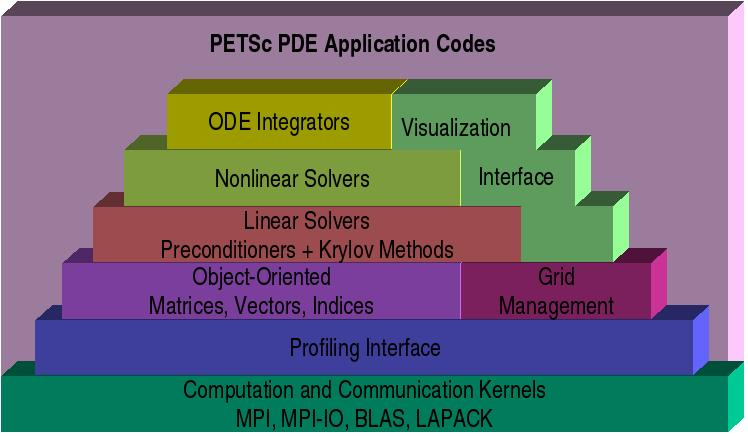
\includegraphics[width=1.0\textwidth]{PETScPyramid.jpg}
 \end{block}

\end{frame}

\begin{frame}[fragile]
\frametitle{Flow Control for a PETSc Application}

\begin{center}
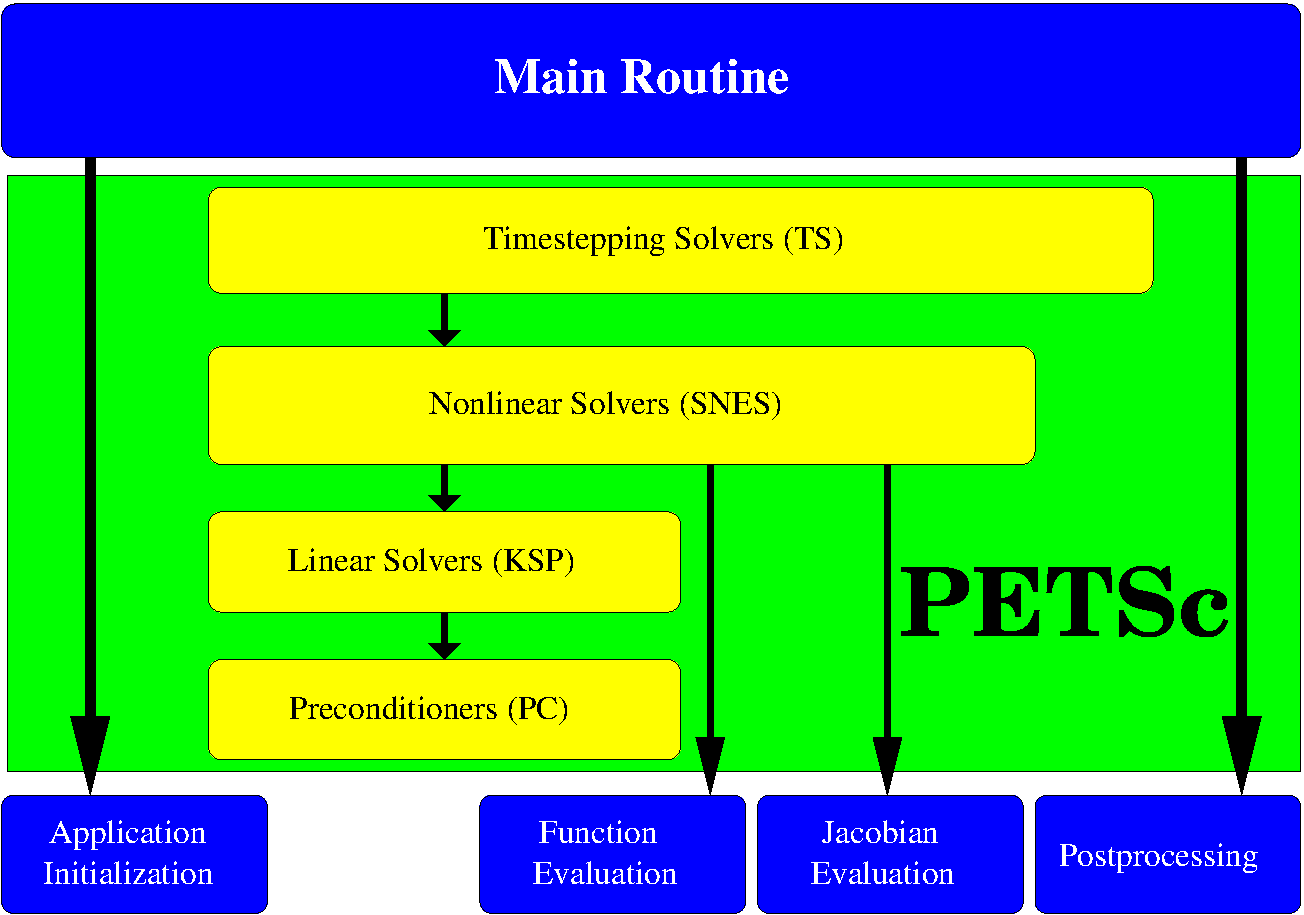
\includegraphics[width=4.0in]{figures/FlowControl}
\end{center}
\end{frame}



\section{PETSc Overview}
\begin{frame}{PETSc}
   \begin{center} \Large \textbf{Vectors and Matrices} \end{center}
\end{frame}



\begin{frame}[fragile]

\frametitle{The Role of PETSc}

\vspace*{\fill}
\begin{minipage}{\linewidth}
\begin{quote}
\Large You want to think about how you decompose your data
structures, how you think about them globally. [...] 

\medskip 

If you
were building a house, you'd start with a set of blueprints
that give you a picture of what the whole house looks
like. You wouldn’t start with a bunch of tiles and say.
``Well I'll put this tile down on the ground, and then I'll
find a tile to go next to it.''

\medskip

But all too many people try to
build their parallel programs by creating the smallest
possible tiles and then trying to have the structure of
their code emerge from the chaos of all these little
pieces. You have to have an organizing principle if
you're going to survive making your code parallel.

\end{quote}

\qquad --- Bill Gropp

\qquad --- http://www.rce-cast.com/Podcast/rce-28-mpich2.html
\end{minipage}
\vspace*{\fill}\vspace*{\fill}

\end{frame}





\begin{frame}[fragile]{PETSc Vectors}

 \begin{block}{Parallel Vector Layout}
   \begin{center}
     \includegraphics[width=0.75\textwidth]{figures/vectors} \\[2em]
   \end{center}
\begin{lstlisting}
  VecCreate(PETSC_COMM_WORLD, &x);
  VecSetSizes(x, PETSC_DECIDE, N);
  VecSetFromOptions(x);
\end{lstlisting}
  \vspace*{2.3cm}
 \end{block}

\end{frame}

\begin{frame}[fragile]{PETSc Vectors}

 \begin{block}{Vector Gather and Scatter}
   \begin{center}
     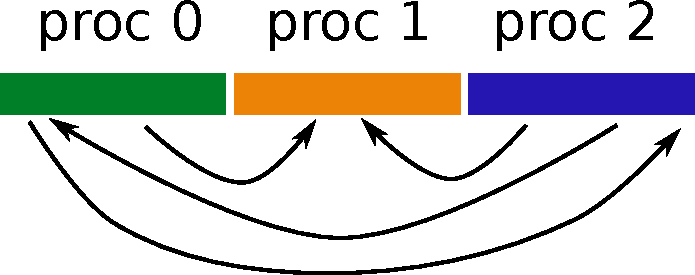
\includegraphics[width=0.75\textwidth]{figures/vectors-scatter} \\[1em]
\begin{lstlisting}
  // y[iy[i]] = x[ix[i]]
  VecScatterCreate(...);
  VecScatterBegin(...);
  VecScatterEnd(...);
\end{lstlisting}
   \end{center}
 \end{block}

\end{frame}

%%%%%%%%%% 


\begin{frame}[fragile]{PETSc Vectors}

 \begin{block}{Vector Reductions}
   \begin{center}
     \includegraphics[width=0.75\textwidth]{figures/vectors-reduce} \\[1.2em]
\begin{lstlisting}
  VecNorm(...);
  VecDot(...);
  VecMax(...);
  ...
\end{lstlisting}
   \end{center}
 \end{block}

\end{frame}


%%%%%%%%%% 

\begin{frame}[fragile]{PETSc Vectors}

 \begin{block}{Local (Sequential) Operations}
  \begin{itemize}
   \item Executed by an arbitrary subset of MPI ranks
   \item Usually involve \lstinline|VecGetArray()/VecRestoreArray()|
  \end{itemize}
 \end{block}

 %\pause
 
 \begin{block}{Collective Operations}
  \begin{itemize}
   \item Must be executed by all processes in the MPI communicator
   \item Involve MPI operations (scatter, gather, reduce, etc.)
  \end{itemize}
 \end{block}

\end{frame}


%
% Matrices (preparing for Linear Solvers)
%


\begin{frame}[fragile]{PETSc Application Integration}

\begin{block}{Sparse Matrices}
\begin{itemize}
  \item \textbf{The} important data type when solving PDEs
  \item Two main phases: 
    \begin{itemize}
     \item Filling with entries (assembly)
     \item Application of its action (e.g.~SpMV)
    \end{itemize}
\end{itemize}
\end{block}
\begin{center}
%\includegraphics[width=2in]{figures/Mat/serialSparseMatrix_bcsstk32}
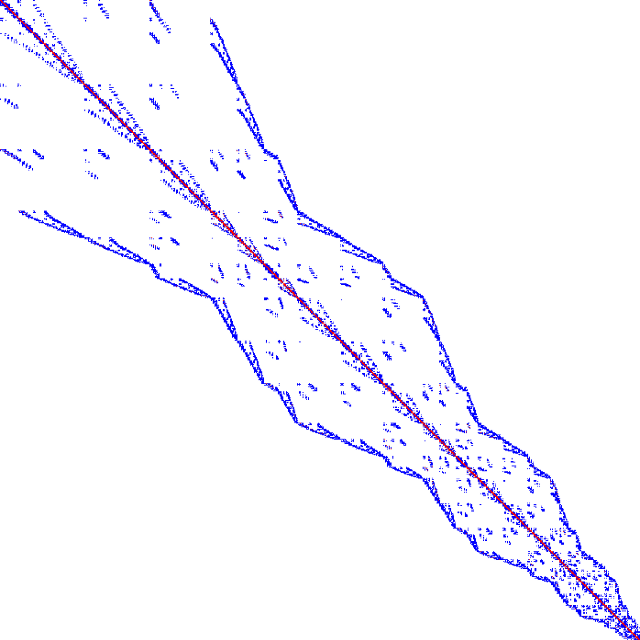
\includegraphics[width=.5\textwidth]{figures/EllipRCMSquare}
\end{center}
\end{frame}



\begin{frame}[fragile]{Matrix Memory Preallocation}
 \begin{block}{PETSc sparse matrices are dynamic data structures}
  \begin{itemize} \vspace*{-0.2cm}
    \item can add additional nonzeros freely
  \end{itemize}
 \end{block}  \vspace*{-0.2cm}

 %\pause
 \begin{block}{Dynamically adding many nonzeros}
  \begin{itemize} \vspace*{-0.2cm}
    \item requires additional memory allocations
    \item requires copies
    \item can kill performance
  \end{itemize}
 \end{block} \vspace*{-0.2cm}

 %\pause
 \begin{block}{Memory preallocation provides}
  \begin{itemize} \vspace*{-0.2cm}
    \item the freedom of dynamic data structures
    \item good performance
  \end{itemize}
 \end{block} \vspace*{-0.2cm}

 %\pause
 \begin{block}{Easiest solution is to replicate the assembly code}
  \begin{itemize} \vspace*{-0.2cm}
    \item Remove computation, but preserve the indexing code
    \item Store set of columns for each row
  \end{itemize}
 \end{block} \vspace*{-0.2cm}

 %\pause
 \begin{block}{Call preallocation routines for all datatypes}
  \begin{itemize} \vspace*{-0.2cm}
    \item \lstinline|MatSeqAIJSetPreallocation()|
    \item \lstinline|MatMPIBAIJSetPreallocation()|
    \item Only the relevant data will be used
  \end{itemize}
\end{block}
\end{frame}




\begin{frame}[fragile]{PETSc Application Integration}

\begin{block}{Sequential Sparse Matrices}
\lstinline|MatSeqAIJSetPreallocation(Mat A, int nz, int nnz[])|
\hbox{\qquad
\vbox{
\begin{itemize}
  \item[nz:] expected number of nonzeros in any row
  \item[nnz(i):] expected number of nonzeros in row i
\end{itemize}
}
}
\end{block}
\begin{center}
%\includegraphics[width=2in]{figures/Mat/serialSparseMatrix_bcsstk32}
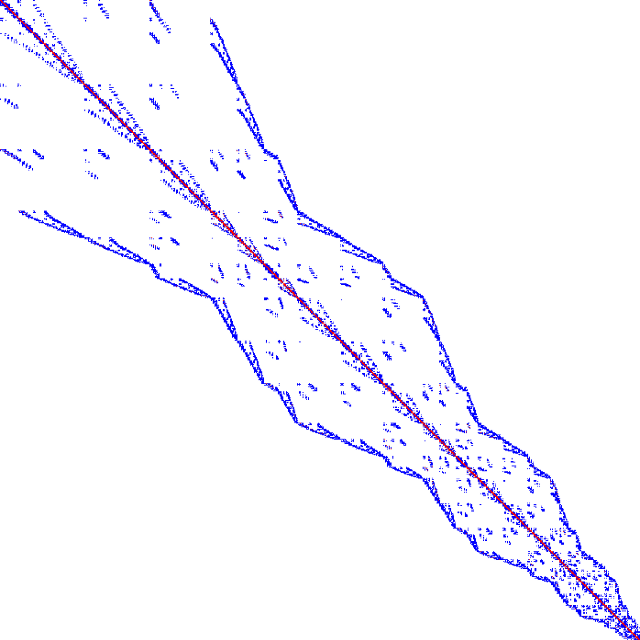
\includegraphics[width=.5\textwidth]{figures/EllipRCMSquare}
\end{center}
\end{frame}

\begin{frame}[fragile]{PETSc Application Integration}

\begin{block}{Parallel Sparse Matrix}
\begin{itemize}
  \item Each process locally owns a submatrix of contiguous global rows
  \item Each submatrix consists of diagonal and off-diagonal parts
\end{itemize}

\begin{center}
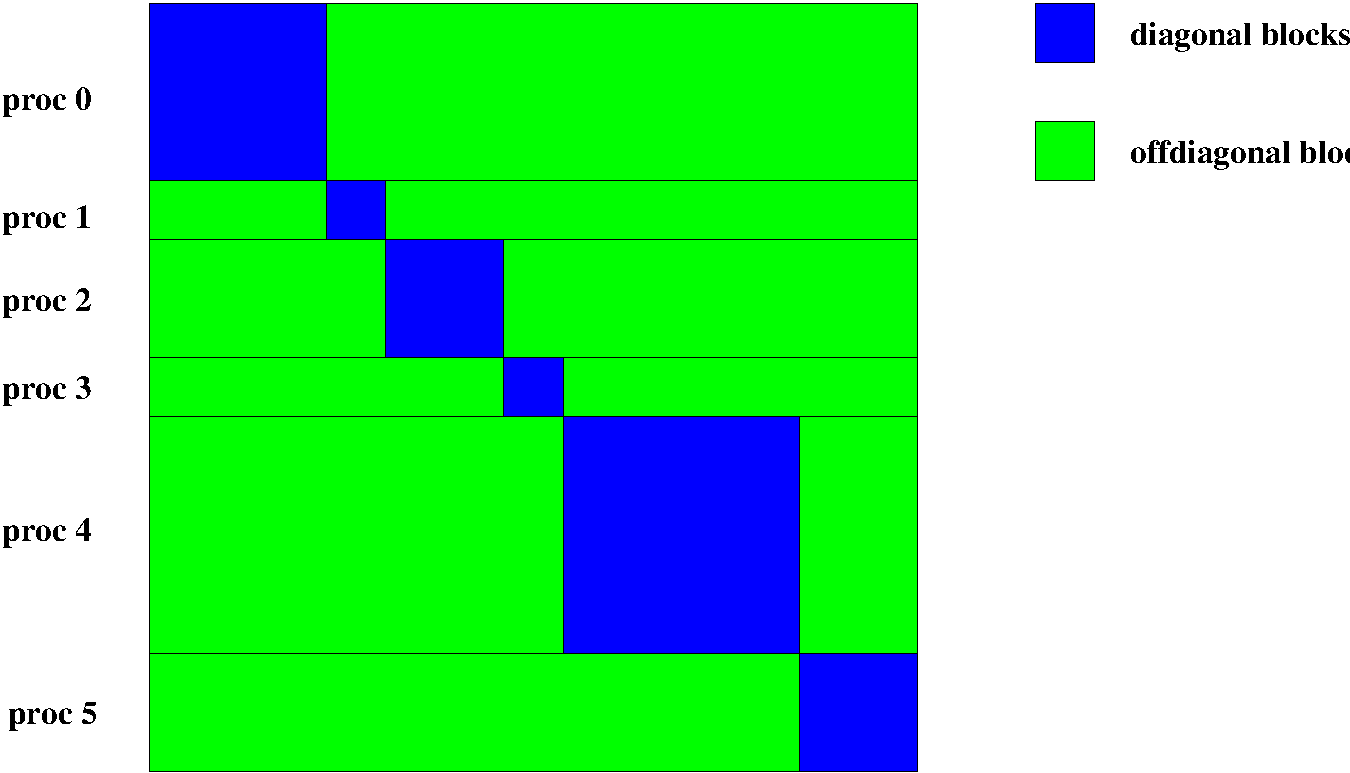
\includegraphics[width=3.in]{figures/Mat/parallelSparseMatrix}
\end{center}

\begin{itemize}
  \item \lstinline|MatGetOwnershipRange(Mat A,int *start,int *end)|
  \begin{itemize}
    \item \lstinline|start|: first locally owned row of global matrix
    \item \lstinline|end-1|: last locally owned row of global matrix
  \end{itemize}
\end{itemize}
\end{block}
\end{frame}


\begin{frame}[fragile]{PETSc Application Integration}

\begin{center}
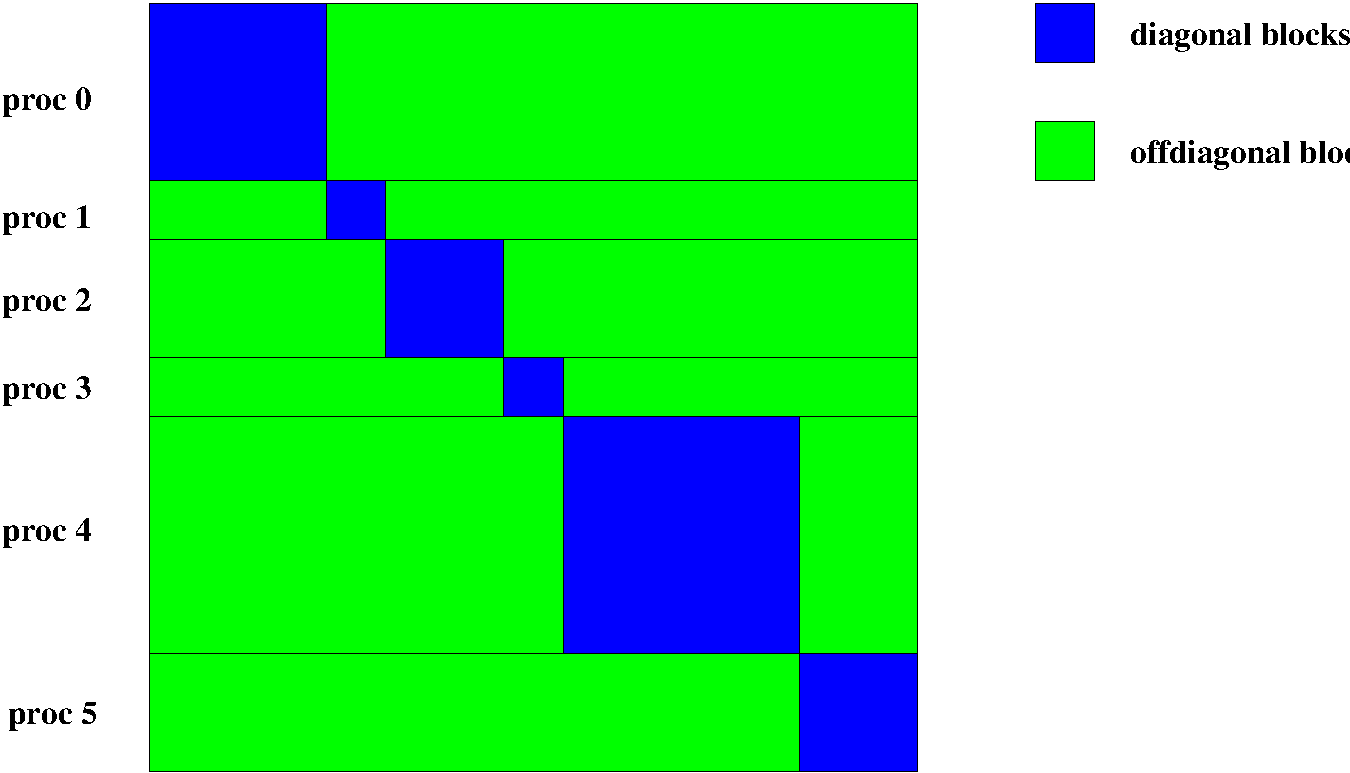
\includegraphics[width=3.in]{figures/Mat/parallelSparseMatrix}
\end{center}

\begin{center}
\begin{tabular}{cc}
\begin{tabular}{c}
\begin{tabular}{|ccc|cc|}
\hline
\multicolumn{3}{|c|}{Proc 2} & \multicolumn{2}{c|}{Proc 3} \\
\hline
25 & 26 & 27 & 28 & 29 \\
20 & 21 & 22 & 23 & 24 \\
15 & 16 & 17 & 18 & 19 \\
\hline
10 & 11 & 12 & 13 & 14 \\
 5 &  6 &  7 &  8 &  9 \\
 0 &  1 &  2 &  3 &  4 \\
\hline
\multicolumn{3}{|c|}{Proc 0} & \multicolumn{2}{c|}{Proc 1} \\
\hline
\end{tabular} \\
Natural numbering
\end{tabular}
& 
\begin{tabular}{c}
\begin{tabular}{|ccc|cc|}
\hline
\multicolumn{3}{|c|}{Proc 2} & \multicolumn{2}{c|}{Proc 3} \\
\hline
21 & 22 & 23 & 28 & 29 \\
18 & 19 & 20 & 26 & 27 \\
15 & 16 & 17 & 24 & 25 \\
\hline
 6 &  7 &  8 & 13 & 14 \\
 3 &  4 &  5 & 11 & 12 \\
 0 &  1 &  2 &  9 & 10 \\
\hline
\multicolumn{3}{|c|}{Proc 0} & \multicolumn{2}{c|}{Proc 1} \\
\hline
\end{tabular}\\
PETSc numbering
\end{tabular}
\end{tabular}
\end{center}

\end{frame}








\begin{frame}[fragile]{PETSc Application Integration}

\begin{block}{Parallel Sparse Matrix}
\vspace{0.5cm}
\hbox{ \quad \vbox{
\begin{lstlisting}
 MatMPIAIJSetPreallocation(Mat A, int dnz, int dnnz[],
                                  int onz, int onnz[]
\end{lstlisting}

\begin{itemize}
  \item[dnz:] expected number of nonzeros in any row in the diagonal block
  \item[dnnz(i):] expected number of nonzeros in row i in the diagonal block
  \item[onz:] expected number of nonzeros in any row in the offdiagonal portion
  \item[onnz(i):] expected number of nonzeros in row i in the offdiagonal portion
\end{itemize}
}}
\end{block}
\end{frame}

\begin{frame}[fragile]{PETSc Application Integration}

\begin{block}{Verifying Preallocation}
\begin{itemize}
  \item Use runtime options 
    \begin{itemize}
      \item \lstinline|-mat_new_nonzero_location_err| 
      \item \lstinline|-mat_new_nonzero_allocation_err|
    \end{itemize}
    
  \item Use runtime option
    \begin{itemize} \item \lstinline|-info| \end{itemize}
  \item Output: \\
\end{itemize}

\end{block}
\begin{lstlisting}[basicstyle=\scriptsize]
[proc #] Matrix size: %d X %d; storage space: %d unneeded, %d used
[proc #] Number of mallocs during MatSetValues( )  is %d
\end{lstlisting}

\begin{center}
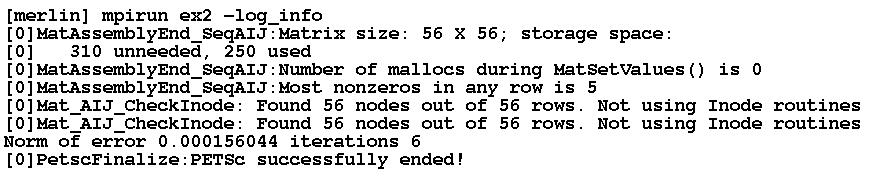
\includegraphics[width=4.in]{figures/logInfoOutput}
\end{center}
\end{frame}

\begin{frame}[fragile]{Block and Symmetric Formats}
  \begin{block}{BAIJ}
    \begin{itemize}
    \item Like AIJ, but uses static block size
    \item Preallocation is like AIJ, but just one index per block
    \end{itemize}
  \end{block}
  
  %\pause
  \begin{block}{SBAIJ}
    \begin{itemize}
    \item Only stores upper triangular part
    \item Preallocation needs number of nonzeros in upper triangular \\
      parts of on- and off-diagonal blocks
    \end{itemize}
  \end{block}
    
  %\pause
  \begin{block}{MatSetValuesBlocked()}
    \begin{itemize}
    \item Better performance with blocked formats
    \item Also works with scalar formats, if \lstinline|MatSetBlockSize()| was called
    \item Variants \lstinline|MatSetValuesBlockedLocal()|, \lstinline|MatSetValuesBlockedStencil()|
    \item Change matrix format at runtime, don't need to touch assembly code
    \end{itemize}
  \end{block}
\end{frame}

\begin{frame}[fragile]{One Way to Set the Elements of a Matrix}

\begin{block}{Simple 3-point stencil for 1D Laplacian}

\begin{lstlisting}
v[0] = -1.0; v[1] = 2.0; v[2] = -1.0;
if (rank == 0) {
  for(row = 0;  row < N; row++) {
    cols[0] = row-1; cols[1] = row; cols[2] = row+1;
    if (row == 0) {
      MatSetValues(A,1,&row,2,&cols[1],&v[1],
                   INSERT_VALUES);
    } else if (row == N-1) {
      MatSetValues(A,1,&row,2,cols,v,INSERT_VALUES);
    } else {
      MatSetValues(A,1,&row,3,cols,v,INSERT_VALUES);
    }
  }
}
MatAssemblyBegin(A,MAT_FINAL_ASSEMBLY);
MatAssemblyEnd(A,MAT_FINAL_ASSEMBLY);
\end{lstlisting}
\end{block}


\end{frame}

\begin{frame}[fragile]{A Better Way to Set the Elements of a Matrix}

\begin{block}{A More Efficient Way}
\small
\begin{lstlisting}
v[0] = -1.0; v[1] = 2.0; v[2] = -1.0;
for(row = start;  row < end; row++) {
  cols[0] = row-1; cols[1] = row; cols[2] = row+1;
  if (row == 0) {
    MatSetValues(A,1,&row,2,&cols[1],&v[1],
                 INSERT_VALUES);
  } else if (row == N-1) {
    MatSetValues(A,1,&row,2,cols,v,INSERT_VALUES);
  } else {
    MatSetValues(A,1,&row,3,cols,v,INSERT_VALUES);
  }
}
MatAssemblyBegin(A, MAT_FINAL_ASSEMBLY);
MatAssemblyEnd(A, MAT_FINAL_ASSEMBLY);
\end{lstlisting}
\end{block}

\begin{block}{Advantages}
 \begin{itemize}
  \item All ranks busy: Scalable!
  \item Amount of code essentially unchanged
 \end{itemize}

\end{block}


\end{frame}



\begin{frame}{Matrices}
  \begin{definition}<1->[Matrix]
    A \alert{matrix} is a linear transformation between finite dimensional vector spaces.
  \end{definition}
  \begin{definition}<1->[Forming a matrix]
    \alert{Forming} or \alert{assembling} a matrix means defining it's action in terms of entries (usually stored in a sparse format).
  \end{definition}
\end{frame}


% Sparse Matrix formats (include benchmark from manual or Jed)
% Matrices in parallel
% Matrix preallocation

\begin{frame}{Matrices}
\begin{block}{Important Matrices}
  \begin{enumerate}
  \item Sparse (e.g.~discretization of a PDE operator)
  \item \alert<2,4>{Inverse of \emph{anything} interesting $B = A^{-1}$}
  \item \alert<4>{Jacobian of a nonlinear function $J y = \lim_{\epsilon \to 0} \frac{F(x + \epsilon y) - F(x)}{\epsilon}$}
  \item \alert<2,4>{Fourier transform $\mathcal{F},\mathcal{F}^{-1}$}
  \item \alert<2,4>{Other fast transforms, e.g. Fast Multipole Method}
  \item \alert<2,4>{Low rank correction $B = A + u v^T$}
  \item \alert<2,4>{Schur complement $S = D - C A^{-1} B$}
  \item \alert<3,4>{Tensor product $A = \sum_e A_x^e \otimes A_y^e \otimes A_z^e$}
  \item \alert<3,4>{Linearization of a few steps of an explicit integrator}
  \end{enumerate}
  \begin{columns}\begin{column}{0.2\textwidth}\end{column}\begin{column}{0.8\textwidth}
  \begin{itemize}
  \item<only@2> These matrices are \alert<2>{dense}.  Never form them.
  \item<only@3>{These are \alert<3>{not very sparse}.}
    Don't form them.
  \item<only@4> {None of these matrices ``have entries''}
  \end{itemize}
\end{column}
\end{columns}
\end{block}
\end{frame}


% \begin{frame}{PETSc}
%    \begin{center} \Large \textbf{What can we do with a matrix \\ which does not have entries?} \\[2em]
%       \visible<2>{\includegraphics[width=0.4\textwidth]{figures/coffee} }
%    \end{center}
% \end{frame}

% 41 distinct slides here




%
% Linear Solvers
%

% Condition number!
\section{Iterative Solvers}
\begin{frame}{PETSc}
   \begin{center} \Large \textbf{Iterative Solvers} \end{center}
\end{frame}

\begin{frame}{Matrices}

\begin{center}
 \em What can we do with a matrix that doesn't have entries?
\end{center}

 %\pause

  \begin{block}{Krylov solvers for $A x = b$}
    \begin{itemize}
    \item Krylov subspace: $\{b, Ab, A^2b, A^3b, \dotsc\}$
    \item Convergence rate depends on the spectral properties of the matrix
      %\begin{itemize}
      %\item Existance of small polynomials $p_n(A) < \epsilon$ where $p_n(0) = 1$.
      %\item condition number $\kappa(A) = \Vert A \Vert \Vert A^{-1} \Vert = \sigma_{\text{max}}/\sigma_{\text{min}}$
      %\item distribution of singular values, spectrum $\Lambda$, pseudospectrum $\Lambda_\epsilon$
%      \item $\epsilon$-pseudospectrum $\Lambda_\epsilon$, spectrum of $A + E$ where $\norm{E} < \epsilon$
      %\end{itemize}
    \item For any popular Krylov method $\mathcal{K}$, there is a matrix
      of size $m$, such that $\mathcal{K}$ outperforms all other methods
      by a factor at least $\mathcal{O}(\sqrt{m})$~[Nachtigal et. al., 1992]%\cite{nachtigal1992fnm}
    \end{itemize}
  \end{block}
  
%\pause

  \begin{block}{Typically...}
    \begin{itemize}
    \item The action $y \gets A x$ can be computed in $\mathcal{O}(m)$
    \item Aside from matrix multiply, the $n^{\text{th}}$ iteration requires at most $\mathcal{O}(mn)$
    \end{itemize}
  \end{block}
\end{frame}


% Dense solvers (reiterate MAGMA-stuff from Day 1)
% Direct solvers (Sparse Gauss, Dissection, etc.)
% Conjugate Gradients
% BiCGStab
\begin{frame}{GMRES}

\begin{block}{Brute force minimization of residual in $\{b,Ab,A^2b,\dotsc\}$}
  \begin{enumerate}
  \item Use Arnoldi to orthogonalize the $n$th subspace, producing
    \[ A Q_n = Q_{n+1} H_n \]
  \item Minimize residual in this space by solving the overdetermined system
    \[ H_n y_n = e_1^{(n+1)} \]
    using $QR$-decomposition, updated cheaply at each iteration.
  \end{enumerate}
\end{block}

%\pause
\begin{block}{Properties}
  \begin{itemize}
  \item Converges in $n$ steps for all right hand sides if there exists a polynomial of degree $n$
    such that $\Vert p_n(A) \Vert < \textit{tol}$ and $p_n(0)=1$.
  \item Residual is monotonically decreasing, robust in practice
  \item Restarted variants are used to bound memory requirements
  \end{itemize}
\end{block}
\end{frame}


\begin{frame}[fragile]{PETSc Solvers}

\begin{block}{Linear Solvers - Krylov Methods}
 \begin{itemize}
  \item Using PETSc linear algebra, just add:
  \begin{lstlisting}[basicstyle=\footnotesize\ttfamily]
KSPSetOperators(KSP ksp, Mat A, Mat M, MatStructure flag)
KSPSolve(KSP ksp, Vec b, Vec x)
  \end{lstlisting}

  \item Can access subobjects
  \begin{lstlisting}[basicstyle=\footnotesize\ttfamily]
KSPGetPC(KSP ksp, PC *pc)
  \end{lstlisting}

  \item Preconditioners must obey PETSc interface
  \begin{itemize}
    \item Basically just the KSP interface
  \end{itemize}

  \item Can change solver dynamically from the command line, \lstinline|-ksp_type|
\end{itemize}
\end{block}

\end{frame}


\begin{frame}{Linear solvers in PETSc KSP}
 \begin{block}{Linear solvers in PETSc KSP (Excerpt)}
  \begin{itemize}
  \item Richardson
  \item Chebychev
  \item Conjugate Gradient
  \item BiConjugate Gradient
  \item Generalized Minimum Residual Variants
  \item Transpose-Free Quasi-Minimum Residual
  \item Least Squares Method
  \item Conjugate Residual
  \end{itemize}
 \end{block}
\end{frame}





%
%%%%% Preconditioners
% 

\section{Preconditioners}
\begin{frame}{PETSc}
   \begin{center} \Large \textbf{Preconditioners} \end{center}
\end{frame}

\subsection{Preconditioning}
\begin{frame}{Preconditioning}
  \begin{block}{Idea: improve the conditioning of the Krylov operator}
    \begin{itemize}
    \item Left preconditioning
      \vspace{-1em}
      \begin{gather*}
        (P^{-1} A) x = P^{-1} b \\
        \{ P^{-1} b, (P^{-1}A) P^{-1} b, (P^{-1}A)^2 P^{-1} b, \dotsc \}
      \end{gather*}
    \item Right preconditioning
      \vspace{-1em}
      \begin{gather*}
        (A P^{-1}) P x = b \\
        \{ b, (P^{-1}A)b, (P^{-1}A)^2b, \dotsc \}
      \end{gather*}
    \item The product $P^{-1}A$ or $A P^{-1}$ is \emph{not} formed.
    \end{itemize}
  \end{block}
  %\begin{definition}[Preconditioner]
      A \emph{preconditioner} $\mathcal{P}$ is a method for constructing a
matrix (just a linear function, not assembled!)  $P^{-1} = \mathcal{P}(A,A_p)$
using a matrix $A$ and extra information $A_p$, such that the spectrum
of $P^{-1}A$ (or $A P^{-1}$) is well-behaved.
   % \end{definition}
\end{frame}

\begin{frame}{Preconditioning}
  \begin{definition}[Preconditioner]
      A \emph{preconditioner} $\mathcal{P}$ is a method for constructing a matrix
      $P^{-1} = \mathcal{P}(A,A_p)$ using a matrix $A$ and extra information $A_p$, such that
      the spectrum of $P^{-1}A$ (or $A P^{-1}$) is well-behaved.
    \end{definition}
    \begin{itemize}
    \item $P^{-1}$ is dense, $P$ is often not available and is not needed
    \item $A$ is rarely used by $\mathcal{P}$, but $A_p = A$ is common
    \item $A_p$ is often a sparse matrix, the ``preconditioning matrix''
    \item Matrix-based: Jacobi, Gauss-Seidel, SOR, ILU(k), LU
    \item Parallel: Block-Jacobi, Schwarz, Multigrid, FETI-DP, BDDC
    \item Indefinite: Schur-complement, Domain Decomposition, Multigrid
    \end{itemize}
\end{frame}


\begin{frame}{Questions to ask when you see a matrix}
  \begin{enumerate}
  \item What do you want to do with it?
    \begin{itemize}
    \item Multiply with a vector
    \item Solve linear systems or eigen-problems
    \end{itemize}
  \item How is the conditioning/spectrum?
    \begin{itemize}
    \item distinct/clustered eigen/singular values?
    \item symmetric positive definite ($\sigma(A) \subset \mathbb{R}^+$)?
    \item nonsymmetric definite ($\sigma(A) \subset \{z \in \mathbb{C} : \mathrm{Re} [z] > 0 \}$)?
    \item indefinite?
    \end{itemize}
  \item How dense is it?
    \begin{itemize}
    \item block/banded diagonal?
    \item sparse unstructured?
    \item denser than we'd like?
    \end{itemize}
  \item Is there a better way to compute $Ax$?
  \item Is there a different matrix with similar spectrum, but nicer properties?
  \item \alert<2>{How can we precondition $A$?}
  \end{enumerate}
\end{frame}

\begin{frame}{Relaxation}
  Split into lower, diagonal, upper parts: \alert{$ A = L + D + U $}
  \begin{block}{Jacobi}
    Cheapest preconditioner: $P^{-1} = D^{-1}$
  \end{block}
  \begin{block}{Successive over-relaxation (SOR)}
    \begin{gather*}
      \left(L + \frac 1 \omega D\right) x_{n+1} = \left[\left(\frac
          1\omega-1\right)D - U\right] x_n + \omega b \\
      P^{-1} = \text{$k$ iterations starting with $x_0=0$}
    \end{gather*}
    \begin{itemize}
    \item Implemented as a sweep
    \item $\omega = 1$ corresponds to Gauss-Seidel
    \item Very effective at removing high-frequency components of residual
    \end{itemize}
  \end{block}
\end{frame}

\begin{frame}[shrink=5]{Factorization}
  \begin{block}{Two phases}
  \begin{itemize}
  \item symbolic factorization: find where fill occurs, only uses sparsity pattern
  \item numeric factorization: compute factors
  \end{itemize}
  \end{block}
  
  
  \begin{block}{LU decomposition}
    \begin{itemize}
    \item Ultimate preconditioner
    \item Expensive, for $m\times m$ sparse matrix with bandwidth $b$, traditionally requires $\mathcal{O}(mb^2)$ time and $\mathcal{O}(mb)$ space.
      \begin{itemize}
      \item Bandwidth scales as $m^{\frac{d-1}{d}}$ in $d$-dimensions
      \item Optimal in 2D: $\mathcal{O}(m \cdot \log m)$ space, $\mathcal{O}(m^{3/2})$ time
      \item Optimal in 3D: $\mathcal{O}(m^{4/3})$ space, $\mathcal{O}(m^2)$ time
      \end{itemize}
    \item Symbolic factorization is problematic in parallel
    \end{itemize}
  \end{block}
  \begin{block}{Incomplete LU}
    \begin{itemize}
    \item Allow a limited number of levels of fill:
      ILU($k$)
    \item Only allow fill for entries that exceed threshold: ILUT
    \item Usually poor scaling in parallel
    \item No guarantees
    \end{itemize}
  \end{block}
\end{frame}

\begin{frame}{1-level Domain decomposition}
  Domain size $L$, subdomain size $H$, element size $h$
  \begin{block}{Overlapping/Schwarz}
    \begin{itemize}\item Solve Dirichlet problems on overlapping
      subdomains
    \item No overlap: $\textit{its} \in \mathcal{O}\big( \frac{L}{\sqrt{Hh}} \big)$
    \item Overlap $\delta$: $\textit{its} \in \big( \frac L {\sqrt{H\delta}} \big)$
    \end{itemize}
  \end{block}
  \begin{block}{Neumann-Neumann}
    \begin{itemize}
    \item Solve Neumann problems on non-overlapping subdomains
    \item $\textit{its} \in \mathcal{O}\big( \frac{L}{H}(1+\log\frac H h) \big)$
    \item Tricky null space issues (floating subdomains)
    \item Need subdomain matrices, net globally assembled matrix.
    \end{itemize}
  \end{block}
  \begin{itemize}
  \item Multilevel variants knock off the leading $\frac L H$
  \item Both overlapping and nonoverlapping with this bound
  \end{itemize}
  % \begin{block}{BDDC and FETI-DP}
  %   \begin{itemize}
  %   \item Neumann problems on subdomains with
  %     coarse grid correction
  %   \item $\textit{its} \in \bigO\big(1 + \log\frac H h \big)$
  %   \end{itemize}
  %   \includegraphics[width=0.7\textwidth]{bddc}
  % \end{block}
\end{frame}

\begin{frame}[shrink=5]{Multigrid}
  \begin{block}{Hierarchy: Interpolation and restriction operators}
    \begin{equation*}
    \mathcal{I}^\uparrow : X_{\text{coarse}} \to X_{\text{fine}} \qquad
    \mathcal{I}^\downarrow :  X_{\text{fine}} \to X_{\text{coarse}}
  \end{equation*}
  \end{block}
  \begin{itemize}
  \item Geometric: define problem on multiple levels, use grid to compute hierarchy
  \item Algebraic: define problem only on finest level, use matrix structure to build hierarchy
  \end{itemize}
  \begin{block}{Galerkin approximation}
    Assemble this matrix: $A_{\text{coarse}} = \mathcal{I}^\downarrow A_{\text{fine}} \mathcal{I}^\uparrow$
  \end{block}
  \begin{block}{Application of multigrid preconditioner ($V$-cycle)}
    \begin{itemize}
    \item Apply pre-smoother on fine level (any preconditioner)
    \item Restrict residual to coarse level with $\mathcal{I}^\downarrow$
    \item Solve on coarse level $A_{\text{coarse}} x = r$
    \item Interpolate result back to fine level with $\mathcal{I}^\uparrow$
    \item Apply post-smoother on fine level (any preconditioner)
    \end{itemize}
  \end{block}
\end{frame}

\begin{frame}{Multigrid convergence properties}
  \begin{itemize}
  \item Textbook: $P^{-1}A$ is spectrally equivalent to identity
    \begin{itemize}
    \item Constant number of iterations to converge up to discretization error
    \end{itemize}
  \item Most theory applies to SPD systems
    \begin{itemize}
    \item variable coefficients (e.g.~discontinuous): low energy interpolants
    \item mesh- and/or physics-induced anisotropy: semi-coarsening/line smoothers
    \item complex geometry: difficult to have meaningful coarse levels
    \end{itemize}
  \item Deeper algorithmic difficulties
    \begin{itemize}
    \item nonsymmetric (e.g.~advection, shallow water, Euler) \\
    \item indefinite (e.g.~incompressible flow, Helmholtz)
    \end{itemize}
  \item Performance considerations
    \begin{itemize}
    \item Aggressive coarsening is critical in parallel
    \item Most theory uses SOR smoothers, ILU often more robust
    \item Coarsest level usually solved semi-redundantly with direct solver
    \end{itemize}
  \item Multilevel Schwarz is essentially the same with different language
    \begin{itemize}
    \item assume strong smoothers, emphasize aggressive coarsening
    \end{itemize}
  \end{itemize}
\end{frame}


% Explain various preconditioners here:
%   - Jacobi, Block-Jacobi
%   - SPAI
%   - ICC/ILU (include symbolic stage)
%   - Multigrid (geometric, algebraic)
%\input{slides/PreconditioningSamples.tex}



% Intermediate summary: Preconditioners for single quantity


\begin{frame}{Splitting for Multiphysics}
  \begin{equation*}
    \begin{bmatrix}
      A & B \\ C & D
    \end{bmatrix}
    \begin{bmatrix}
      x \\ y
    \end{bmatrix}
    =
    \begin{bmatrix}
      f \\ g
    \end{bmatrix}
  \end{equation*}
  \begin{itemize}\item Relaxation: \lstinline|-pc_fieldsplit_type| \newline
    \lstinline| [additive,multiplicative,symmetric_multiplicative]|
    \begin{equation*}
      \begin{bmatrix}
        A & \\  & D
      \end{bmatrix}^{-1} \qquad 
      \begin{bmatrix}
        A & \\ C & D
      \end{bmatrix}^{-1} \qquad
      \begin{bmatrix}
        A & \\  & \mathbf{1}
      \end{bmatrix}^{-1}
      \left(
        \mathbf{1} -
        \begin{bmatrix}
          A & B \\ & \mathbf{1}
        \end{bmatrix}
        \begin{bmatrix}
          A & \\ C & D
        \end{bmatrix}^{-1}
      \right)
    \end{equation*}
    \begin{itemize}
    \item Gauss-Seidel inspired, works when fields are loosely coupled
    \end{itemize}
  \item Factorization: \lstinline|-pc_fieldsplit_type schur|
    \begin{align*}
      \begin{bmatrix}
        A & B \\ & S
      \end{bmatrix}^{-1}
      \begin{bmatrix}
        \mathbf{1} & \\ CA^{-1} & \mathbf{1}
      \end{bmatrix}^{-1}, \qquad
      S = D - C A^{-1} B
    \end{align*}
    \begin{itemize}
    \item robust (exact factorization), can often drop lower block
    \item how to precondition $S$ which is usually dense?
      \begin{itemize}
      \item interpret as differential operators, use approximate commutators
      \end{itemize}
    \end{itemize}
  \end{itemize}
\end{frame}

% Compose preconditioners for multiple fields (Fun with Matt)




%
%%%%% Distributed Arrays
%


\section{Distributed Arrays}
\begin{frame}{PETSc}
   \begin{center} \Large \textbf{Distributed Arrays} \end{center}
\end{frame}

\begin{frame}[fragile]{Distributed Array}

  \begin{block}{Interface for topologically structured grids}
  \end{block}

  \begin{block}{Defines (topological part of) a finite-dimensional function space}
    \begin{itemize} 
      \item Get an element from this space: \lstinline|DMCreateGlobalVector()| 
    \end{itemize}
  \end{block}

  \begin{block}{Provides parallel layout}
  \end{block}

  \begin{block}{Refinement and coarsening}
    \begin{itemize}
      \item \lstinline|DMRefineHierarchy()| 
    \end{itemize}
  \end{block}

  \begin{block}{Ghost value coherence}
    \begin{itemize}
       \item \lstinline|DMGlobalToLocalBegin()|
     \end{itemize}
  \end{block}

  \begin{block}{Matrix preallocation}
       \begin{itemize}
         \item \lstinline|DMCreateMatrix()| (formerly \lstinline|DMGetMatrix()|) 
       \end{itemize}
  \end{block}
\end{frame}

\begin{frame}
\frametitle{Ghost Values}

\begin{block}{To evaluate a local function $f(x)$, each process requires}
\begin{itemize}
  \item its local portion of the vector $x$
  \item its {\color{cyan}ghost values}, bordering portions of $x$ owned by neighboring processes
\end{itemize}
\end{block}

\begin{center}
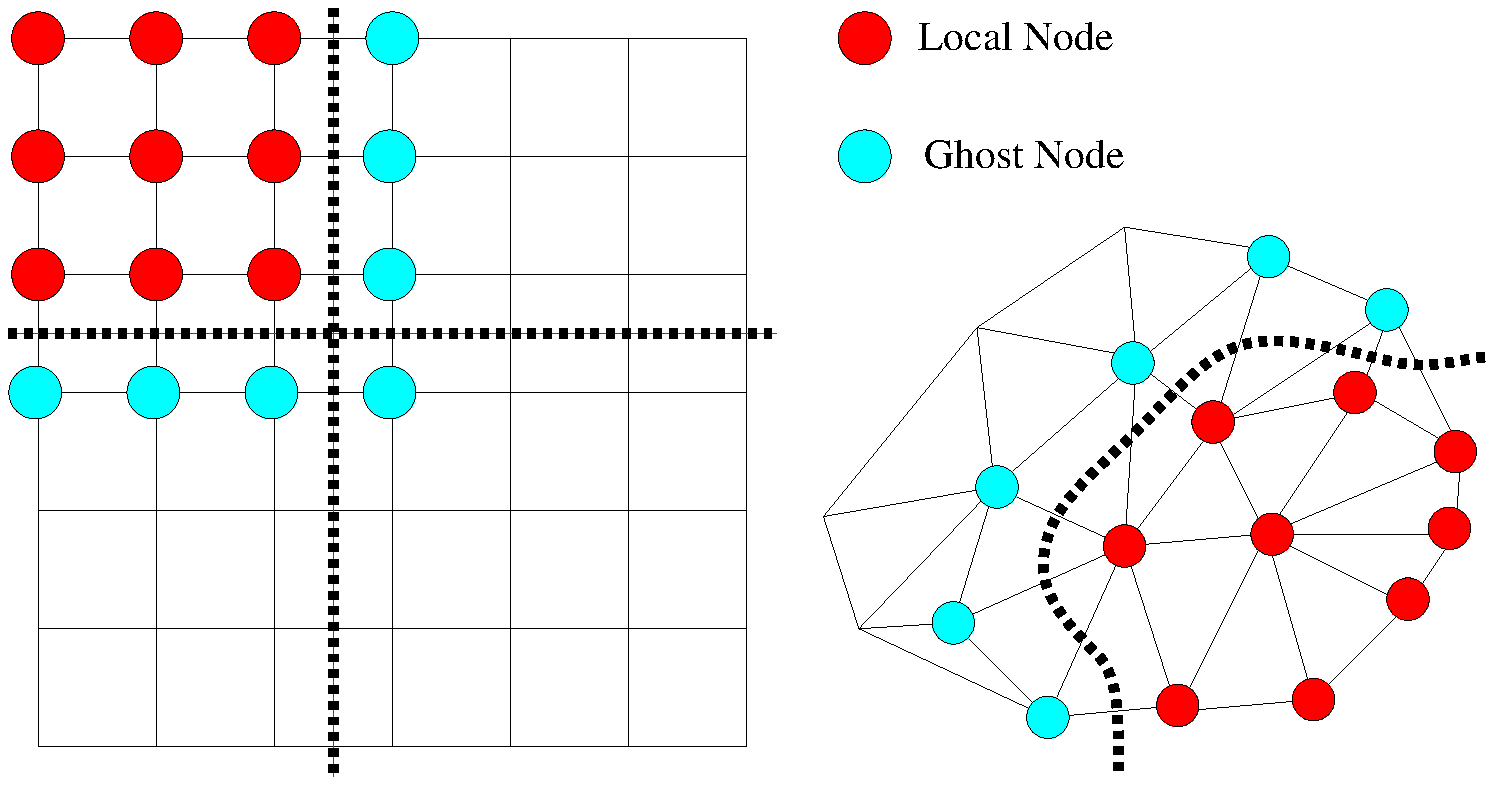
\includegraphics[width=4in]{figures/GhostValues}
\end{center}

\end{frame}

\begin{frame}{DMDA Global Numberings}

\begin{center}
\begin{tabular}{cc}
\begin{tabular}{c}
\begin{tabular}{|ccc|cc|}
\hline
\multicolumn{3}{|c|}{Proc 2} & \multicolumn{2}{c|}{Proc 3} \\
\hline
25 & 26 & 27 & 28 & 29 \\
20 & 21 & 22 & 23 & 24 \\
15 & 16 & 17 & 18 & 19 \\
\hline
10 & 11 & 12 & 13 & 14 \\
 5 &  6 &  7 &  8 &  9 \\
 0 &  1 &  2 &  3 &  4 \\
\hline
\multicolumn{3}{|c|}{Proc 0} & \multicolumn{2}{c|}{Proc 1} \\
\hline
\end{tabular} \\
Natural numbering
\end{tabular}
& 
\begin{tabular}{c}
\begin{tabular}{|ccc|cc|}
\hline
\multicolumn{3}{|c|}{Proc 2} & \multicolumn{2}{c|}{Proc 3} \\
\hline
21 & 22 & 23 & 28 & 29 \\
18 & 19 & 20 & 26 & 27 \\
15 & 16 & 17 & 24 & 25 \\
\hline
 6 &  7 &  8 & 13 & 14 \\
 3 &  4 &  5 & 11 & 12 \\
 0 &  1 &  2 &  9 & 10 \\
\hline
\multicolumn{3}{|c|}{Proc 0} & \multicolumn{2}{c|}{Proc 1} \\
\hline
\end{tabular}\\
PETSc numbering
\end{tabular}
\end{tabular}
\end{center}
\end{frame}

\begin{frame}{DMDA Global vs. Local Numbering}

\begin{itemize}
  \item {\bf Global}: Each vertex has a unique id, belongs on a unique process

  \item {\bf Local}: Numbering includes vertices from neighboring processes
  \begin{itemize}
    \item These are called {\color{cyan}ghost} vertices
  \end{itemize}
\end{itemize}

\begin{center}
\begin{tabular}{cc}
\begin{tabular}{c}
\begin{tabular}{|ccc|cc|}
\hline
\multicolumn{3}{|c|}{Proc 2} & \multicolumn{2}{c|}{Proc 3} \\
\hline
 X &  X &  X &  X &  X \\
 X &  X &  X &  X &  X \\
{\color{cyan}12} & {\color{cyan}13} & {\color{cyan}14} & {\color{cyan}15} &  X \\
\hline
 8 &  9 & 10 & {\color{cyan}11} &  X \\
 4 &  5 &  6 & {\color{cyan}7} &  X \\
 0 &  1 &  2 & {\color{cyan}3} &  X \\
\hline
\multicolumn{3}{|c|}{Proc 0} & \multicolumn{2}{c|}{Proc 1} \\
\hline
\end{tabular} \\
Local numbering
\end{tabular}
& 
\begin{tabular}{c}
\begin{tabular}{|ccc|cc|}
\hline
\multicolumn{3}{|c|}{Proc 2} & \multicolumn{2}{c|}{Proc 3} \\
\hline
21 & 22 & 23 & 28 & 29 \\
18 & 19 & 20 & 26 & 27 \\
15 & 16 & 17 & 24 & 25 \\
\hline
 6 &  7 &  8 & 13 & 14 \\
 3 &  4 &  5 & 11 & 12 \\
 0 &  1 &  2 &  9 & 10 \\
\hline
\multicolumn{3}{|c|}{Proc 0} & \multicolumn{2}{c|}{Proc 1} \\
\hline
\end{tabular}\\
Global numbering
\end{tabular}
\end{tabular}
\end{center}
\end{frame}




\begin{frame}[fragile]{PETSc Vectors}

 \begin{block}{Parallel Vector Layout}
   \begin{center}
     \includegraphics[width=0.75\textwidth]{figures/vectors} \\[2em]
   \end{center}
\begin{lstlisting}
  VecCreate(PETSC_COMM_WORLD, &x);
  VecSetSizes(x, PETSC_DECIDE, N);
  VecSetFromOptions(x);
\end{lstlisting}
  \vspace*{2.3cm}
 \end{block}

\end{frame}

\begin{frame}[fragile]{PETSc Vectors}

 \begin{block}{Vector Gather and Scatter}
   \begin{center}
     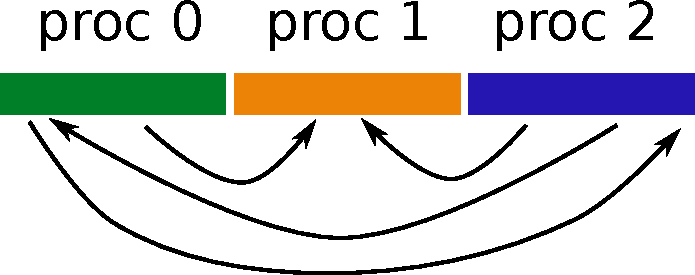
\includegraphics[width=0.75\textwidth]{figures/vectors-scatter} \\[1em]
\begin{lstlisting}
  // y[iy[i]] = x[ix[i]]
  VecScatterCreate(...);
  VecScatterBegin(...);
  VecScatterEnd(...);
\end{lstlisting}
   \end{center}
 \end{block}

\end{frame}

%%%%%%%%%% 


\begin{frame}[fragile]{PETSc Vectors}

 \begin{block}{Vector Reductions}
   \begin{center}
     \includegraphics[width=0.75\textwidth]{figures/vectors-reduce} \\[1.2em]
\begin{lstlisting}
  VecNorm(...);
  VecDot(...);
  VecMax(...);
  ...
\end{lstlisting}
   \end{center}
 \end{block}

\end{frame}


%%%%%%%%%% 

\begin{frame}[fragile]{PETSc Vectors}

 \begin{block}{Local (Sequential) Operations}
  \begin{itemize}
   \item Executed by an arbitrary subset of MPI ranks
   \item Usually involve \lstinline|VecGetArray()/VecRestoreArray()|
  \end{itemize}
 \end{block}

 %\pause
 
 \begin{block}{Collective Operations}
  \begin{itemize}
   \item Must be executed by all processes in the MPI communicator
   \item Involve MPI operations (scatter, gather, reduce, etc.)
  \end{itemize}
 \end{block}

\end{frame}

\begin{frame}{Updating Ghosts}

\begin{block}{Two-step Process for Updating Ghosts}
 \begin{itemize}
  \item enables overlapping computation and communication
 \end{itemize}
\end{block}
 

\begin{block}{\lstinline|DMGlobalToLocalBegin(dm, gvec, mode, lvec)|}
  \begin{itemize}
    \item \lstinline|gvec| provides the data 
    \item \lstinline|mode| is either \lstinline|INSERT_VALUES| or \lstinline|ADD_VALUES|
    \item \lstinline|lvec| holds the local and ghost values
  \end{itemize}
\end{block}

\begin{block}{\lstinline|DMGlobalToLocalEnd(dm, gvec, mode, lvec)|}
  \begin{itemize}
    \item Finishes the communication
  \end{itemize}
\end{block}

\medskip

\begin{block}{Reverse Process}
  \begin{itemize}
   \item Via \lstinline|DMLocalToGlobalBegin()| and \lstinline|DMLocalToGlobalEnd()|.
  \end{itemize}
\end{block}
 
\end{frame}

\begin{frame}
\frametitle{DMDA Stencils}

\begin{block}{Available Stencils}
%  \begin{itemize}
%   \item {\color{blue}box} stencil
%   \item {\color{blue}star} stencil
%  \end{itemize}
\end{block}

\begin{center}
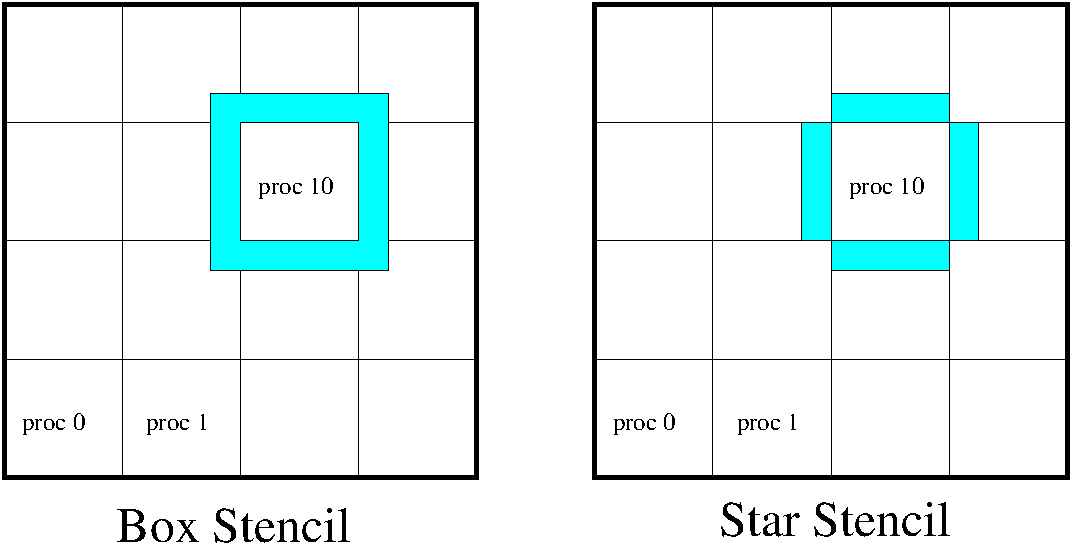
\includegraphics[width=0.95\textwidth]{figures/DA/Stencils}
\end{center}
\end{frame}

\begin{frame}[fragile]
\frametitle{Creating a DMDA}

{\small \lstinline|DMDACreate2d(comm, xbdy, ybdy, type, M, N, m, n|, \\
\qquad\qquad\qquad \qquad  \lstinline|dof, s, lm[], ln[], DA *da)|}

\begin{block}{\lstinline|xbdy,ybdy|: Specifies periodicity or ghost cells}
  \vspace*{-0.2cm}
  \begin{itemize}
    \item \lstinline|DMDA_BOUNDARY_NONE|, \lstinline|DMDA_BOUNDARY_GHOSTED|, \lstinline|DMDA_BOUNDARY_MIRROR|, \lstinline|DMDA_BOUNDARY_PERIODIC|
  \end{itemize}
\end{block}

\vspace*{-0.3cm}
\begin{block}{\lstinline|type|}
  \vspace*{-0.2cm}
  \begin{itemize}
    \item Specifies stencil: \lstinline|DMDA_STENCIL_BOX| or \lstinline|DMDA_STENCIL_STAR|
  \end{itemize}
\end{block}

\vspace*{-0.3cm}
\begin{block}{\lstinline|M,N|}
  \vspace*{-0.2cm}
  \begin{itemize}
    \item Number of grid points in x/y-direction
  \end{itemize}
\end{block}

\vspace*{-0.3cm}
\begin{block}{\lstinline|m,n|}
  \vspace*{-0.2cm}
  \begin{itemize}
    \item Number of processes in x/y-direction
  \end{itemize}
\end{block}

\vspace*{-0.3cm}
\begin{block}{\lstinline|dof|}
  \vspace*{-0.2cm}
  \begin{itemize}
    \item Degrees of freedom per node
  \end{itemize}
\end{block}

\vspace*{-0.3cm}
\begin{block}{\lstinline|s|}
  \vspace*{-0.2cm}
  \begin{itemize}
    \item The stencil width
  \end{itemize}
\end{block}

\vspace*{-0.3cm}
\begin{block}{\lstinline|lm,ln|}
  \vspace*{-0.2cm}
  \begin{itemize}
    \item Alternative array of local sizes
    \item Use \lstinline|NULL| for the default
  \end{itemize}
\end{block}

\end{frame}

\begin{frame}[fragile]{Working with the Local Form}

\begin{block}{Wouldn't it be nice if we could just write our code for the natural numbering?}
 
 \only<1>{
\begin{center}
\begin{tabular}{cc}
\begin{tabular}{c}
\begin{tabular}{|ccc|cc|}
\hline
\multicolumn{3}{|c|}{Proc 2} & \multicolumn{2}{c|}{Proc 3} \\
\hline
25 & 26 & 27 & 28 & 29 \\
20 & 21 & 22 & 23 & 24 \\
15 & 16 & 17 & 18 & 19 \\
\hline
10 & 11 & 12 & 13 & 14 \\
 5 &  6 &  7 &  8 &  9 \\
 0 &  1 &  2 &  3 &  4 \\
\hline
\multicolumn{3}{|c|}{Proc 0} & \multicolumn{2}{c|}{Proc 1} \\
\hline
\end{tabular} \\
Natural numbering
\end{tabular}
& 
\begin{tabular}{c}
\begin{tabular}{|ccc|cc|}
\hline
\multicolumn{3}{|c|}{Proc 2} & \multicolumn{2}{c|}{Proc 3} \\
\hline
21 & 22 & 23 & 28 & 29 \\
18 & 19 & 20 & 26 & 27 \\
15 & 16 & 17 & 24 & 25 \\
\hline
 6 &  7 &  8 & 13 & 14 \\
 3 &  4 &  5 & 11 & 12 \\
 0 &  1 &  2 &  9 & 10 \\
\hline
\multicolumn{3}{|c|}{Proc 0} & \multicolumn{2}{c|}{Proc 1} \\
\hline
\end{tabular}\\
PETSc numbering
\end{tabular}
\end{tabular}
\end{center}
\vspace*{1cm}
    }
    
    
 \only<2>{
  \begin{itemize}
  \item Yes, that's what \lstinline|DMDAVecGetArray()| is for.
  \end{itemize}
  }
  
  \end{block}
  
  \only<2>{
 \begin{block}{DMDA offers \emph{local} callback functions}
    \begin{itemize}
      \item \lstinline|FormFunctionLocal()|, set by \lstinline|DMDASetLocalFunction()|
      \item \lstinline|FormJacobianLocal()|, set by \lstinline|DMDASetLocalJacobian()|
    \end{itemize}
 \end{block}

 
 \begin{block}{Evaluating the nonlinear residual $F(x)$}
    \begin{itemize}
      \item Each process evaluates the local residual
      \item PETSc assembles the global residual automatically
        \begin{itemize}
        \item Uses \lstinline|DMLocalToGlobal()| method
        \end{itemize}
    \end{itemize}
 \end{block}
 }

\end{frame}

\begin{frame}[fragile]{Thinking of Extensions}

\begin{block}{Multiple Unknowns per Grid Node}
  \begin{itemize}
   \item Example 1: Displacements $u_x$, $u_y$
   \item Example 2: Velocity components, Pressure
   \item Typical in a multiphysics setting
  \end{itemize}
\end{block}

\begin{block}{Multiple Unknowns in a Distributed Setting}
  \begin{itemize}
   \item Robust abstract concepts important
   \item Lots of bookkeeping
   \item All done by PETSc
  \end{itemize}

\end{block}

\end{frame}


\begin{frame}[fragile]{Thinking of Extensions}

\begin{center}
 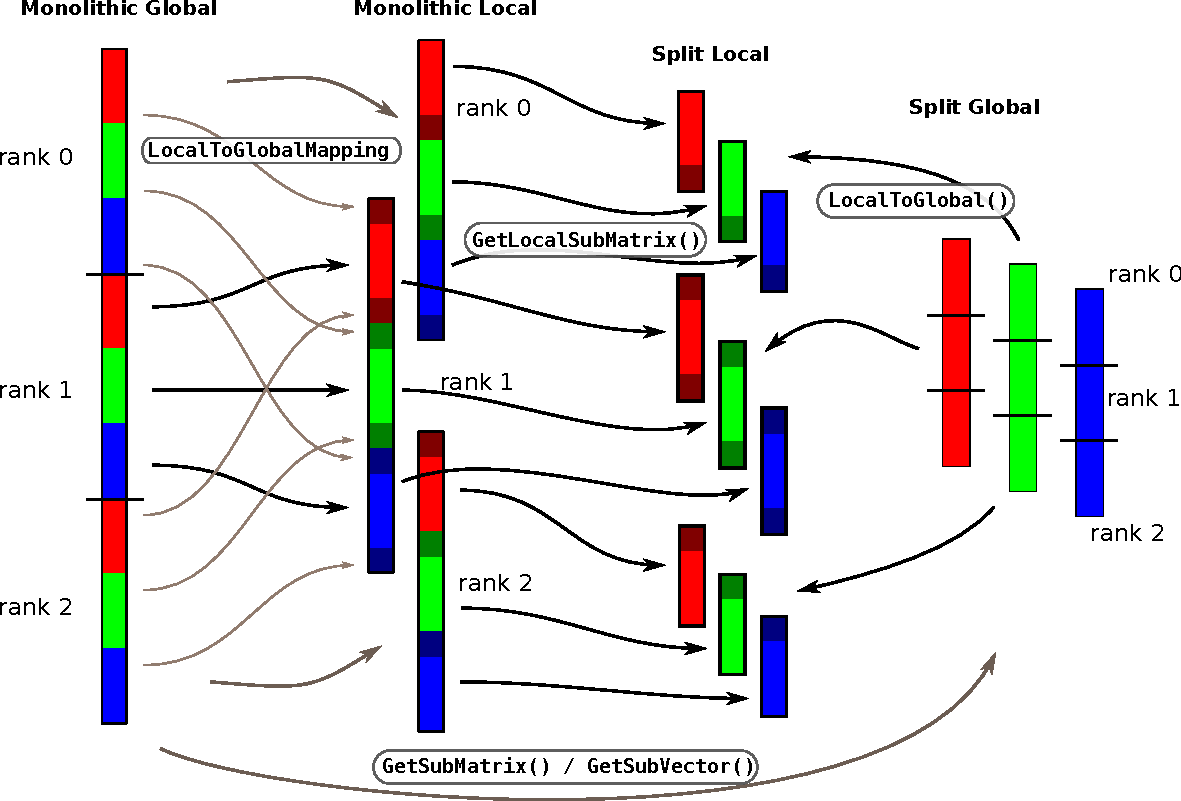
\includegraphics[width=\textwidth]{figures/localspaces}
\end{center}


\end{frame}

\begin{frame}[fragile]
\frametitle{DA Local Function}

\begin{block}{User-provided Function for Nonlinear Residual in 2D}
\begin{lstlisting}
  PetscErrorCode (*lfunc)(DMDALocalInfo *info,
                          Field **x, Field **r,
                          void *ctx)
\end{lstlisting}

\begin{tabular}{lp{8.3cm}}
  \lstinline|info| & All layout and numbering information \\
  \lstinline|x|    & The current solution \newline
     \emph{ Notice that it is a multidimensional array} \\
  \lstinline|r|    & The residual \\
  \lstinline|ctx|  & The user context passed to \lstinline|DMSetApplicationContext()| or to SNES \\
\end{tabular}


\bigskip

The local DMDA function is activated by calling
\begin{itemize}
 \item \lstinline|SNESSetDM(snes,dm)|
 \item \lstinline|SNESSetFunction(snes, r, SNESDAFormFunction, ctx)|
\end{itemize}
\end{block}
\end{frame}











%
%%%%% Preconditioners
% 


%

\begin{frame}[fragile]
\frametitle{PETSc Objects}
\begin{block}{Sample Code}
  \begin{lstlisting}
    Mat A;
    PetscInt m,n,M,N;
    MatCreate(comm,&A);
    MatSetSizes(A,m,n,M,N);      /* or PETSC_DECIDE */ 
    MatSetOptionsPrefix(A,"foo_");
    MatSetFromOptions(A);
    /* Use A */
    MatView(A,PETSC_VIEWER_DRAW_WORLD);
    MatDestroy(A);
  \end{lstlisting}
  \end{block}
  
  \begin{block}{Remarks}
  \begin{itemize}
  \item \lstinline|Mat| is an opaque object (pointer to incomplete type)
    \begin{itemize}
     \item Assignment, comparison, etc, are cheap
    \end{itemize}
  \item What's up with this ``Options'' stuff?
    \begin{itemize}
    \item We will discuss this later...
    \end{itemize}
  \end{itemize}
  
\end{block}
\end{frame}

\begin{frame}{Basic PetscObject Usage}

\begin{block}{Every object in PETSc supports a basic interface}
\vspace{0.3cm}
\begin{tabular}{|r|l|}
\hline
Function & Operation \\
\hline
\texttt{Create()}               & create the object \\
\texttt{Get/SetName()}          & name the object \\
\texttt{Get/SetType()}          & set the implementation type \\
\texttt{Get/SetOptionsPrefix()} & set the prefix for all options \\
\texttt{SetFromOptions()}       & customize object from command line \\
\texttt{SetUp()}                & perform other initialization \\
\texttt{View()}                 & view the object \\
\texttt{Destroy()}              & cleanup object allocation \\
\hline
\end{tabular}

\end{block}

\begin{block}{Also, all objects support the \lstinline|-help| option.}\end{block}

\end{frame}


\begin{frame}[fragile]{PETSc Options}
\begin{block}{Ways to set options}
  \begin{itemize}
  \item Command line
  \item Filename in the third argument of \lstinline|PetscInitialize()|
  \item \lstinline|~/.petscrc|
  \item \lstinline|$PWD/.petscrc|
  \item \lstinline|$PWD/petscrc|
  \item \lstinline|PetscOptionsInsertFile()|
  \item \lstinline|PetscOptionsInsertString()|
  \item \lstinline|PETSC_OPTIONS| environment variable
  \item command line option \lstinline|-options_file [file]|
  \end{itemize}
\end{block}
\end{frame}


\begin{frame}[fragile]{PETSc Options}

\begin{block}{Example of Command Line Control}
  %\lstinline|$> cd $PETSC_DIR/src/snes/examples/tutorials && make ex5}| \\
  \begin{itemize}
  \item \lstinline|$> ./ex5 -da_grid_x 10 -da_grid_y 10 -par 6.7| \\
      \lstinline|       -snes_monitor -{ksp,snes}_converged_reason| \\
      \lstinline|       -snes_view|
  \item \lstinline|$> ./ex5 -da_grid_x 10 -da_grid_y 10 -par 6.7| \\
      \lstinline|       -snes_monitor -{ksp,snes}_converged_reason| \\
      \lstinline|       -snes_view -mat_view_draw -draw_pause 0.5|
  \item \lstinline|$> ./ex5 -da_grid_x 10 -da_grid_y 10 -par 6.7| \\
      \lstinline|       -snes_monitor -{ksp,snes}_converged_reason| \\
      \lstinline|       -snes_view -mat_view_draw -draw_pause 0.5| \\
      \lstinline|       -pc_type lu -pc_factor_mat_ordering_type natural|
  \item Use \lstinline|-help| to find other ordering types
\end{itemize}
\end{block}
\end{frame}



%\section{Application Integration}
%\begin{frame}{PETSc}
%   \begin{center} \Large \textbf{Application Integration} \end{center}
%\end{frame}

%\begin{frame}{Application Integration}

\begin{block}{Be willing to experiment with algorithms}
  \begin{itemize}
    \item No optimality without interplay between physics and algorithmics
  \end{itemize}
\end{block}

\begin{block}{Adopt flexible, extensible programming}
  \begin{itemize}
    \item Algorithms and data structures not hardwired
  \end{itemize}
\end{block}

\begin{block}{Be willing to play with the real code}
  \begin{itemize}
    \item Toy models have limited usefulness
    \item But make test cases that run quickly
  \end{itemize}
\end{block}

\begin{block}{If possible, profile before integration}
  \begin{itemize}
    \item Automatic in PETSc
  \end{itemize}
\end{block}

\end{frame}

%\begin{frame}[fragile]{Incorporating PETSc into Existing Codes}
  \begin{block}{PETSc does not seize \lstinline|main()|, does not control output}   \end{block} \vspace*{-0.4cm}
  %\pause
  \begin{block}{Propogates errors from underlying packages, flexible}   \end{block} \vspace*{-0.4cm}
  %\pause
  \begin{block}{Nothing special about \lstinline|MPI_COMM_WORLD|}   \end{block} \vspace*{-0.4cm}
  %\pause
  \begin{block}{Can wrap existing data structures/algorithms}
    \begin{itemize} \vspace*{-0.2cm}
    \item \lstinline|MatShell|, \lstinline|PCShell|, full implementations
    \item \lstinline|VecCreateMPIWithArray()|
    \item \lstinline|MatCreateSeqAIJWithArrays()|
    \item Use an existing semi-implicit solver as a preconditioner
    \item Usually worthwhile to use native PETSc data structures \\
      unless you have a good reason not to
    \end{itemize}
  \end{block} \vspace*{-0.4cm}
  %\pause
  \begin{block}{Uniform interfaces across languages}
    \begin{itemize} \vspace*{-0.2cm}
    \item C, C++, Fortran 77/90, Python, MATLAB
    \end{itemize}
  \end{block} \vspace*{-0.4cm}
  %\pause
  \begin{block}{Do not have to use high level interfaces (e.g.~SNES, TS, DM)}
    \begin{itemize} \vspace*{-0.2cm}
    \item but PETSc can offer more if you do, like MFFD and SNES Test
    \end{itemize}
  \end{block}
\end{frame}

%\begin{frame}{Integration Stages}

\begin{block}{\color{red} Version Control}
  \begin{itemize} \vspace*{-0.1cm}
    \item It is impossible to overemphasize
  \end{itemize} \vspace*{-0.1cm}
\end{block}

\begin{block}{Initialization}
  \begin{itemize} \vspace*{-0.1cm}
    \item Linking to PETSc
  \end{itemize} \vspace*{-0.1cm}
\end{block}

\begin{block}{Profiling}
  \begin{itemize} \vspace*{-0.1cm}
    \item Profile {\color{red} before} changing
    \item Also incorporate command line processing
  \end{itemize} \vspace*{-0.1cm}
\end{block}

\begin{block}{Linear Algebra}
  \begin{itemize} \vspace*{-0.1cm}
    \item First PETSc data structures
  \end{itemize} \vspace*{-0.1cm}
\end{block}

\begin{block}{Solvers}
  \begin{itemize} \vspace*{-0.1cm}
    \item Very easy after linear algebra is integrated
  \end{itemize}
\end{block}

\end{frame}




%%%%%%%%%%%%%%%%%%%%%%%%%%%%


%

\begin{frame}{Typical PETSc Operations}
 
  \begin{block}{``Sparse'' Linear Algebra}
   \begin{itemize}
    \item Sparse Matrix-Vector Operations (on-node)
    \item Vector Operations (on and across nodes)
    \item Only on small patches: Dense Operations (\emph{small} matrices)
   \end{itemize}
  \end{block}

   \begin{center}
     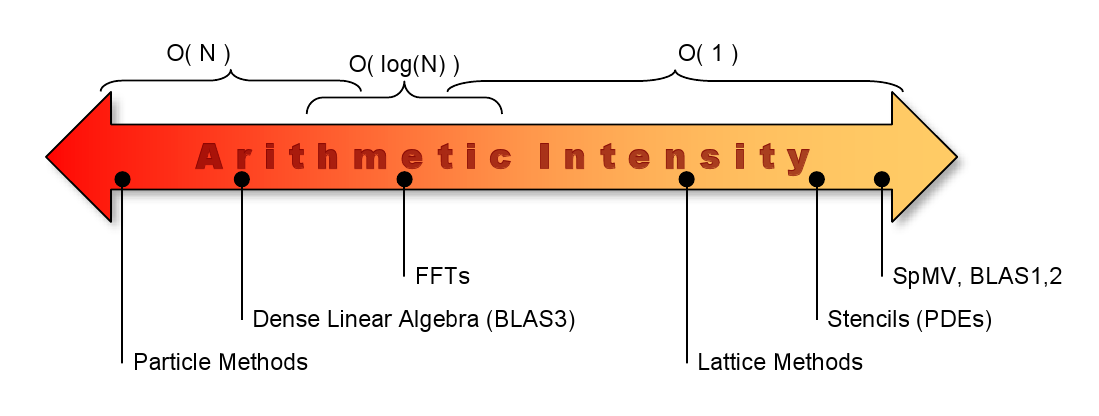
\includegraphics[width=0.95\textwidth]{figures/OlikerArithmeticIntensity.png} \\
    $\leftarrow$ Look at FLOPs \hspace{3cm} Look at Mem-BW $\rightarrow$
   \end{center}

\end{frame}





%%%% Conclusion


\section{Summary}
\begin{frame}{Summary}
 
 \begin{block}{PETSc Can Help You}
  \begin{itemize}
   \item solve algebraic and DAE problems in your application area
   \item rapidly develop efficient parallel code, can start from examples
   \item develop new solution methods and data structures
   \item debug and analyze performance
   \item advice on software design, solution algorithms, and performance
   \item \centering \texttt{petsc-\{users,dev,maint\}@mcs.anl.gov}

  \end{itemize}
 \end{block}

 %\pause
 \begin{block}{You Can Help PETSc}
  \begin{itemize}
   \item report bugs and inconsistencies, or if you think there is a better way
   \item tell us if the documentation is inconsistent or unclear
   \item consider developing new algebraic methods as plugins, contribute if your idea works
  \end{itemize}
 \end{block}

\end{frame}
